\subsection{Company Image} \label{company_image}
%Philipp and Janine

The company image is a very important KPI to measure the company reputation. The company image is the sum of many small activities which leaves a footprint that can be recognized with the company. Single activities can improve or destroy the \textit{companyImage} (\gls{cI}) from the point of view of individuals. The goal of a high valued company image is of course monetary benefit. Therefore, activities which tend to increase the \textit{companyImage} are not for free and it is always a difficult assessment whether to invest in a certain activity or not. In the game we concentrated on factors which can be realistically and interestingly be influenced by the player.

% cost table alternative
\begin{table}[]
\centering
\begin{tabular}{|l|r|r|r|}
\hline
\multicolumn{1}{|l|}{\textbf{Action}} & \multicolumn{1}{l}{\textbf{Costs in CapCoins}} & \multicolumn{1}{l}{} & \multicolumn{1}{l|}{} \\
CSR (in \% of profit)     & depending on profit &                   & \\
Support Refugee Projects  & 1000        &                   & \\
  & \underline{newspaper} & \underline{TV}      &  \underline{Online} \\
Marketing Campaigns       & 5000                & 10000             & 100000 \\
\hline
\end{tabular}
\caption{Cost campaigns}
\label{cost_campaigns}
\end{table}

\begin{table}[]
\begin{tabular}{|l|r|r|r|}
\hline
\multicolumn{1}{|l|}{\textbf{Action}}             & \multicolumn{1}{l|}{\textbf{Points}} & \multicolumn{1}{l|}{}       & \multicolumn{1}{l|}{}   \\
\textbf{Social engagement}        &       &       &  \\
\underline{CSR (in \% of profit)} & 0     &       &  \\
\textless 1\%                     & 1     &       &  \\
1\% \textless 2\%                 & 2     &       &  \\
2\% \textless 5\%                 & 3     &       &  \\
5\% \textless{}                   & 4     &       &  \\
\underline{Support refugee projects}  &   &       &  \\
never                             & 0     &       &  \\
1 project per year                & 1     &       &  \\
at least 2 projects per year      & 2     &       &  \\
&  &  &  \\
\textbf{Marketing Campaigns}  & \textbf{Newspaper} & \textbf{Television} & \textbf{Online} \\
\underline{Promote environmental friendly supplier}   & & & \\
never                             & 0    & 0      & 0 \\
1 time per year                   & 1    & 1.5    & 2 \\
at least 2 times per year         & 1.5  & 2      & 2.5 \\
\underline{Promote environmental friendly production} & & & \\
never                             & 0    & 0      & 0 \\
1 time per year                   & 1    & 1.5    & 2 \\
at least 2 times per year         & 1.5  & 2      & 2.5 \\
\underline{Green marketing campaign} & & & \\
never                             & 0    & 0      & 0 \\
1 time per year                   & 1    & 1.5    & 2 \\
2 times per year                  & 2    & 3      & 4 \\
3 times per year                  & 3    & 4.5    & 6 \\
at least 4 times per year         & 3.5  & 5      & 6.5  \\
\underline{Diversity Campaign}    & & & \\
never                             & 0    & 0      & 0 \\
1 time per year                   & 0.5  & 1      & 1.5  \\
at least 2 times per year         & 1    & 1.5    & 2 \\
\underline{Promote Products} & & & \\
never                             & 0    & 0      & 0 \\
1 time per year                   & 1.5  & 2      & 2.5  \\
2 times per year                  & 3    & 4      & 5.5  \\
3 times per year                  & 4.5  & 6      & 8 \\
at least 4 times per year         & 5    & 6.5    & 8.5  \\
\hline
\end{tabular}
\caption{Actions influencing the Company Image}
\label{calculation_CI}
\end{table}

The total sum of the above possible choices is the total \textit{companyImage}. The score can reach values from 0 to 28 as it is the case for the \textit{employeeSatisfaction}. In order to build also here a more realistic representation we figured out that the marginal benefit of an increase of the \textit{companyImage} increases with the collected amount of points. Therefore, we manipulated also this formula and came up with the function that can be seen in figure \ref{fig:scaling}.

%is now on a single page, how can we solve this? but only by surrounding it with figure it is possible to give it a caption. 
\begin{figure}
    \centering
    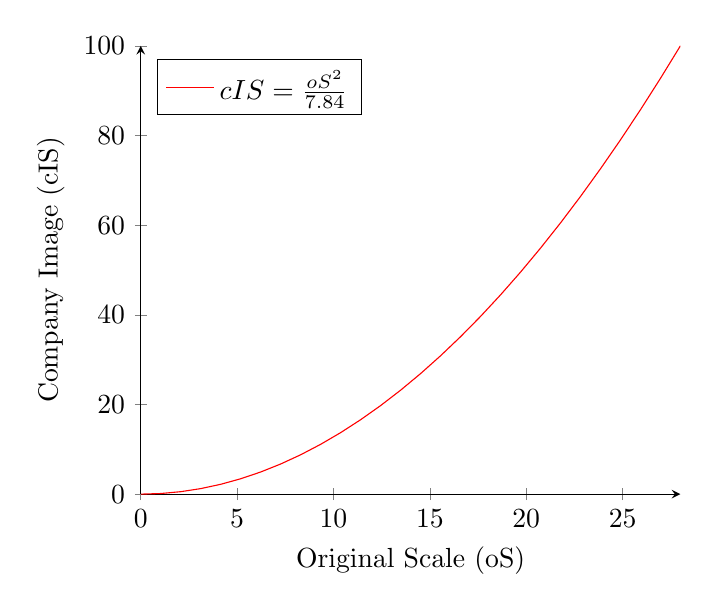
\begin{tikzpicture}
    \begin{axis}[
        axis lines = left,
        xlabel = Original Scale (\gls{oS}),
        ylabel = Company Image  (cIS),
        grid style = dashed,
        legend pos=north west
    ]
    \addplot [
        domain=0:28, 
        samples=28, 
        color=red,
    ]
    {x^2/7.84};
    \addlegendentry{$cIS=\frac{oS^2}{7.84}$}
    \end{axis}
    \end{tikzpicture}
    \caption{Scaling function companyImage}
    \label{fig:scaling}
\end{figure}

The original scale of 0 to 28 is squared and divided by the factor of 7.84 in order to map the original scale on a scale of 0 to 100. In this case the rational behind the mapping is the fact that little activities do not have such  a big influence on the overall \textit{companyImage}. When a company starts to combine all its activities it can generate huge impact and publicity which leads to a strong increase of the \textit{companyImage}.